\documentclass[11pt]{article}
\usepackage[margin=1in]{geometry}
\usepackage{amsmath,amssymb,amsthm}
\usepackage{graphicx}
\usepackage{microtype}
\usepackage[hidelinks]{hyperref}

\newtheorem{theorem}{Theorem}
\newtheorem{lemma}{Lemma}
\newcommand{\F}{\mathcal F}
\newcommand{\Hh}{\mathcal H}

\title{A Shannon--Haar Counterexample to\\
Interpolation-Unitary Normalization}
\author{Candidate result for arXiv:math/0604619, Problem 4}
\date{27 August 2026}

\begin{document}
\maketitle

\begin{center}
\fbox{\parbox{0.9\textwidth}{\textbf{Status.}
Candidate counterexample, likely valid, pending expert review. The result gives
a negative answer to Problem 4 of Larson's source paper.}}
\end{center}

\section{Source problem}

Let
\[
  (Df)(x)=\sqrt2\,f(2x),\qquad (Tf)(x)=f(x-1)
\]
on $L^2(\mathbb R)$.  For dyadic orthonormal wavelets $\psi,\eta$, the
interpolation unitary $V_\psi^\eta$ is the unitary determined by
\[
 V_\psi^\eta D^jT^k\psi=D^jT^k\eta
 \qquad(j,k\in\mathbb Z).
\]
Larson asks whether $V_\psi^\eta$ must normalize $\{D,T\}'$
\cite[Problem 4, p.~28]{Larson2006}.

\begin{figure}[ht]
\centering
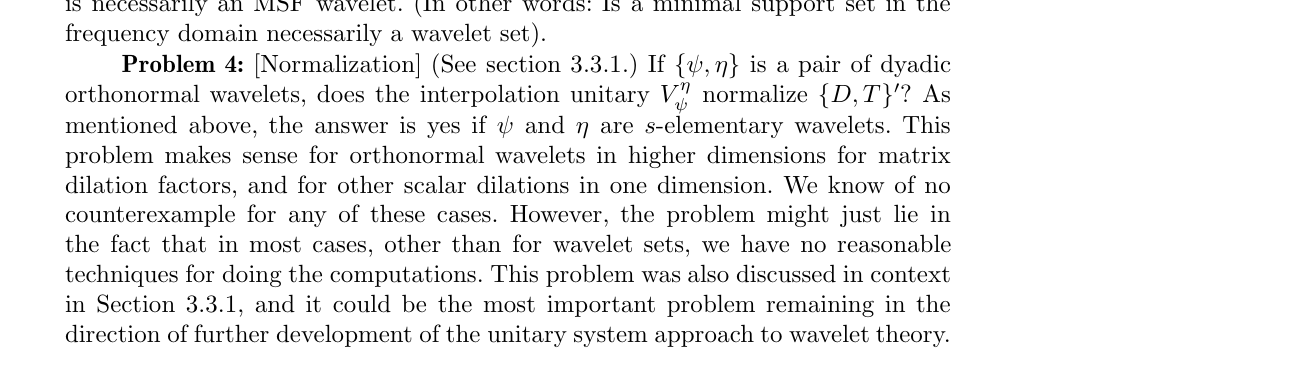
\includegraphics[width=\textwidth]{figures/open_problem_crop.png}
\caption{Problem 4 in the source PDF, page 28.}
\end{figure}

The source proves the Fourier-side commutant characterization
\begin{equation}\label{eq:commutant}
 \F\{D,T\}'\F^{-1}
 =\{M_h:h\in L^\infty(\mathbb R),\ h(s)=h(2s)\text{ a.e.}\}
\end{equation}
\cite[Theorem 4.1, pp.~12--13]{Larson2006}.

\section{Definitions and the proposed family}

Use the unitary Fourier transform
\[
 \widehat f(s)=\frac1{\sqrt{2\pi}}\int_{\mathbb R}e^{-isx}f(x)\,dx.
\]
The Shannon wavelet $\psi_S$ is defined by
\[
 \widehat\psi_S=\frac1{\sqrt{2\pi}}\mathbf1_E,
 \qquad E=[-2\pi,-\pi)\cup[\pi,2\pi).
\]
The argument applies to every dyadic orthonormal wavelet $\eta$ such that
$\widehat\eta\ne0$ almost everywhere.  For an explicit example, take the
standard Haar wavelet
\[
 \psi_H=\mathbf1_{[0,1/2)}-\mathbf1_{[1/2,1)}.
\]
Both are dyadic orthonormal wavelets.  A direct integration gives
\begin{equation}\label{eq:haarft}
 \widehat\psi_H(s)
 =\frac{(1-e^{-is/2})^2}{is\sqrt{2\pi}},
\end{equation}
with the value at $s=0$ defined by continuity.  In particular,
$\widehat\psi_H$ is nonzero almost everywhere: its zeros form a countable set.

Let $p$ be the $2\pi$-periodic half-torus mask
\begin{equation}\label{eq:p}
 p(s)=\mathbf1_{[\pi,2\pi)}(s\bmod 2\pi).
\end{equation}
Then $p$ is not $2$-dilation-periodic.  Indeed, for
$s\in(\pi/2,\pi)$ one has $p(s)=0$ and $p(2s)=1$.

\section{Idea of the proof}

The positive-frequency projection is a member of the commutant because its
symbol is invariant under $s\mapsto2s$.  On the two Shannon frequency bands,
that projection is exactly the periodic mask $p$.  Periodicity means that $p$
acts through a translate-coefficient Fourier series.  The interpolation unitary
preserves those coefficients when it replaces every Shannon translate by the
corresponding target-wavelet translate, so the conjugated projection sends the
target mother wavelet to $p\widehat\eta$.

If the interpolation unitary normalized the commutant, this conjugated
projection would be $M_h$ for a dilation-periodic $h$.  Its action on the target
mother wavelet would force $h=p$ almost everywhere because
$\widehat\eta\ne0$ almost everywhere.  This is impossible because $p$ is not
dilation-periodic.

\section{Formal result and proof}

\begin{theorem}\label{thm:main}
Let $\eta$ be any dyadic orthonormal wavelet satisfying
$\widehat\eta\ne0$ almost everywhere, and let $V=V_{\psi_S}^{\eta}$ be the
interpolation unitary from the Shannon wavelet to $\eta$.  Then $V$ does not
normalize $\{D,T\}'$.  In particular, this holds for $\eta=\psi_H$, so Problem
4 in \cite{Larson2006} has a negative answer.
\end{theorem}

\begin{proof}
Work in the Fourier domain and write
\[
 \widehat V=\F V\F^{-1},\qquad
 P_+=M_q,\qquad q=\mathbf1_{(0,\infty)}.
\]
Since $q(2s)=q(s)$ almost everywhere, \eqref{eq:commutant} gives
$P_+\in\F\{D,T\}'\F^{-1}$.

On the Shannon support $E$, the functions $q$ and $p$ agree.  Hence
\begin{equation}\label{eq:onshannon}
 P_+\widehat\psi_S=M_p\widehat\psi_S.
\end{equation}
Let $(c_k)_{k\in\mathbb Z}$ be the Fourier coefficients of $p$, with signs
chosen so that
\[
 p(s)=\sum_{k\in\mathbb Z}c_ke^{-iks}
 \quad\text{in }L^2([0,2\pi)).
\]
The fixed-scale translates of either wavelet are orthonormal.  Therefore their
synthesis maps are isometries from $\ell^2(\mathbb Z)$ onto their respective
closed translate spans.  Applying the finite Fourier sums first and then taking
the $L^2$ limit gives
\begin{align}
 M_p\widehat\psi_S
   &=\sum_{k\in\mathbb Z}c_k\widehat T^k\widehat\psi_S,
   \label{eq:seriesS}\\
 M_p\widehat\eta
   &=\sum_{k\in\mathbb Z}c_k\widehat T^k\widehat\eta.
   \label{eq:serieseta}
\end{align}
By the defining property of the interpolation unitary,
$\widehat V\widehat T^k\widehat\psi_S
=\widehat T^k\widehat\eta$.  Since $\widehat V$ is unitary,
\eqref{eq:onshannon}--\eqref{eq:serieseta} imply
\begin{equation}\label{eq:transport}
 \widehat V P_+\widehat\psi_S=M_p\widehat\eta.
\end{equation}

Set $R=\widehat V P_+\widehat V^*$.  Since
$\widehat V^*\widehat\eta=\widehat\psi_S$, equation
\eqref{eq:transport} says
\begin{equation}\label{eq:Reta}
 R\widehat\eta=M_p\widehat\eta.
\end{equation}
Suppose, toward a contradiction, that $V$ normalizes $\{D,T\}'$.  Then $R$
belongs to the Fourier-side commutant.  By \eqref{eq:commutant}, $R=M_h$ for
some $h\in L^\infty(\mathbb R)$ satisfying $h(s)=h(2s)$ almost everywhere.
Equation \eqref{eq:Reta} yields
\[
 (h-p)\widehat\eta=0\quad\text{a.e.}
\]
The hypothesis $\widehat\eta\ne0$ almost everywhere gives $h=p$ almost
everywhere.  This contradicts the failure of
$p(s)=p(2s)$ on $(\pi/2,\pi)$.  Therefore $V$ does not normalize the
commutant.  Formula \eqref{eq:haarft} verifies the hypothesis for the explicit
choice $\eta=\psi_H$.
\end{proof}

\section{Verification notes}

The proof was attacked at the following convention-sensitive points.
\begin{itemize}
\item If the opposite orientation for $V_\psi^\eta$ is adopted, the argument
uses the inverse conjugation.  A unitary normalizes an algebra if and only if
its adjoint does, so the conclusion is unchanged.
\item A Fourier-series sign reversal only reindexes the translate coefficients.
The mask $p$ is real, and the transported multiplier identity is unchanged.
\item Values at the endpoints of the half-torus intervals and at the countable
zero set of $\widehat\psi_H$ are null-set issues.
\item No numerical evidence is used; the counterexample is exact.
\end{itemize}
The independent step-by-step verifier report is included as
\texttt{verification.md}.  Current verdict: \textbf{likely valid}.

\section{Scope and novelty check}

This counterexample addresses exactly the one-dimensional dyadic question.  It
does not make claims about other scalar dilations or higher-dimensional matrix
dilations.

A bounded novelty search on 27 August 2026 covered the run's lightweight
registry, solution, attempt, and proof-gap indexes, together with
exact and close arXiv/web searches for ``interpolation unitary'', ``normalize
commutant'', ``Shannon Haar'', and Larson's Problem 4.  The search found the
source paper and the related 2006 exposition arXiv:math/0604615, but no later
explicit solution or counterexample.  This was not an exhaustive
citation-database search; novelty is therefore provisional.

\section{Human-review recommendation}

Send to a wavelet/operator-algebra expert.  The highest-value review step is to
check equations \eqref{eq:seriesS}--\eqref{eq:transport}, namely that the same
periodic Fourier coefficients synthesize the masked Shannon and target mother
wavelets and are transported term by term by the interpolation unitary.

\begin{thebibliography}{9}
\bibitem{Larson2006}
D. R. Larson,
\emph{Unitary systems and wavelet sets},
arXiv:math/0604619 (2006).
\end{thebibliography}

\end{document}
